\chapter{Xuen: Implémentation}

\section{Signaux}

\subsection{Hiérarchie}
\label{sec:sig-hierarchy}

La figure \ref{sec:sig-hierarchy} présente la hiérarchie formée par les différentes classes de signaux. Cette section aborde plus en détails les spécificités de chacune d'elles.

\begin{figure}[h]
	\centering
	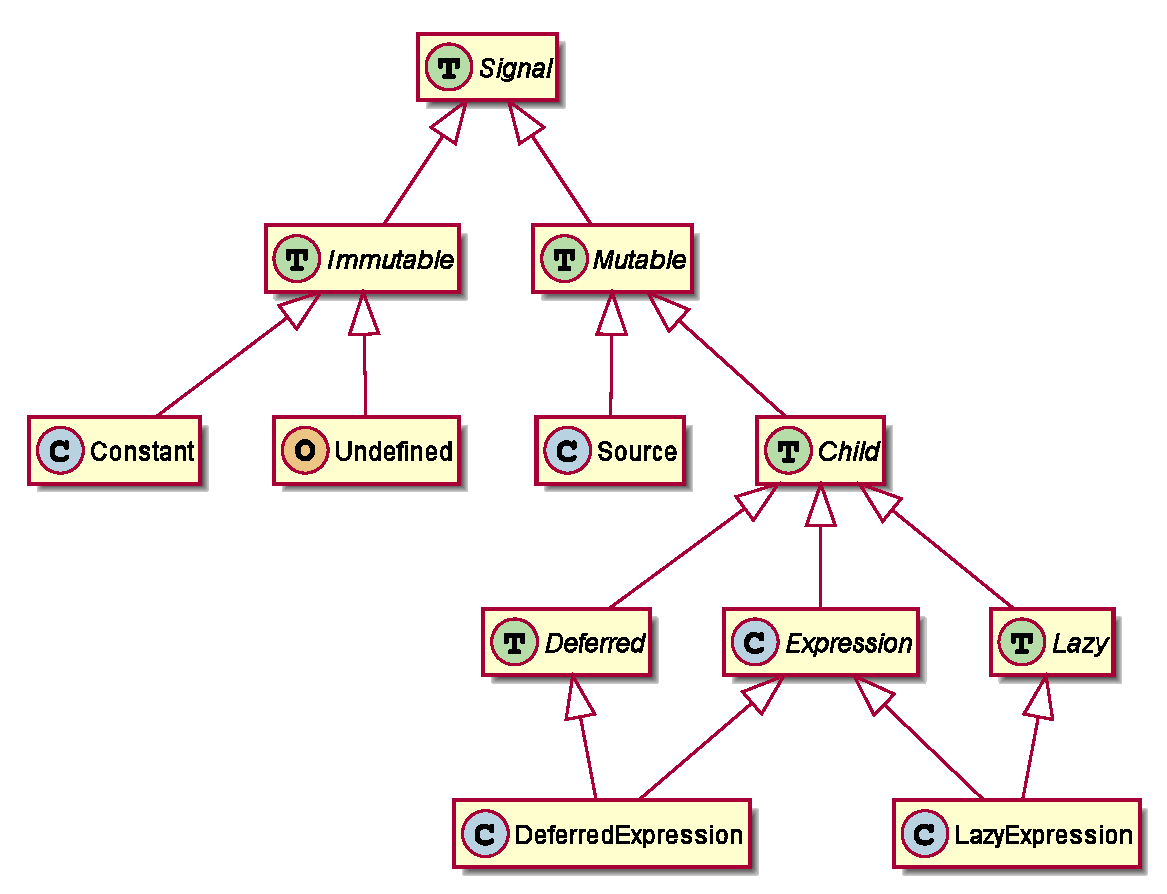
\includegraphics[width=10cm]{img/sig_hierarchy.eps}
	\caption{Hiérarchie des signaux}
	\label{fig:sig-hierarchy}
\end{figure}

\subsubsection{\texttt{Signal}}

Le trait racine de la hiérarchie expose les opérations communes à tous les signaux: accès à la valeur courante et opération de transformation. C'est une interface générique qui ne précise aucune sémantique particulière pour le signal. Elle est ainsi adaptée lorsque le type exact de signal manipulé n'est pas important, ce qui est généralement le cas.

\subsubsection{\texttt{Immutable}}

Cette première division distingue les signaux dont la valeur change au cours du temps de ceux pour lesquels la valeur reste constante.

\subsubsection{\texttt{Mutable}}

\subsubsection{\texttt{Lazy}}

\subsection{Implémentation des opérateurs monadiques}

\textit{CONTRAIREMENT À REACTIVEX, PAS DE CLASSES, MAIS UTILISATION DES EXPRESSIONS}

\subsection{Modèle push, pull ou hybride}

Deux modes de fonctionnement sont généralement décrit pour des systèmes fonctionnels-réactifs: \emph{push} et \emph{pull}.

L'approche \emph{push} se base sur les changements apportés aux signaux sources pour recalculer tous les signaux enfants qui en dépendent. Dans l'approche \emph{pull}, c'est l'accès aux signaux enfants qui provoque le calcul des valeurs intermédiaires jusqu'aux signaux sources. Dans les deux cas, des opérations potentiellement inutiles ou redondantes sont effectuées.

L'approche mixte \emph{push-pull} se base sur une approche principalement \emph{pull} où l'accès à l'état d'un signal déclenche son évaluation, auquel vient s'ajouter un mécanisme de \emph{mémoïsation} qui maintient l'état courant du signal après son calcul. L'invalidation de ces caches se fait ensuite selon une approche \emph{push}: un changement d'état des signaux sources est notifié à toutes les dépendances de façon récursive.

\textit{DEVELOPPEMENT DES AVANTAGES}

\subsection{Utilisation dans un environnement parallèle}

\textit{Pas de threads en JavaScript, donc un problème que côté serveur. Bien que le système fonctionne sur la JVM, il n'a pas été testé de façon étendue dans un contexte multi-thread; actuellement half-baked: les Signaux eux-même sont en principe thread-safe (aka invalidation / recalcul / etc) mais le système en entier n'est pas réellement étudié (dead-lock de signaux interdépendant?). Est-ce que utile au projet puisqu'on le use-case principal est celui du framework web côté client? Quid des observeurs et de la sémantique exactly-once pour une bloc de mutation atomic{} ?}

\section{Framework web}
